\documentclass[11pt,a4paper]{article}
\usepackage{pdfpages}
\usepackage{helvet}
\usepackage{graphicx}
\usepackage{color}
\usepackage{pgf}
\usepackage{rotating}
\usepackage{eurosym}
\usepackage{wrapfig}
\usepackage{setspace}
\usepackage{eso-pic}
\usepackage{subfig}
\usepackage{afterpage}
\usepackage{sidecap}
%\usepackage[numbers]{natbib}
\usepackage{enumitem}
%\usepackage{natbib}
%\usepackage{aas_macros}
%\usepackage{url}
\usepackage{hyperref}
\usepackage{multirow}
\usepackage[percent]{overpic}
\usepackage{booktabs}
\usepackage{latexsym}
\usepackage{pdfpages}
\usepackage{tabularx}

%\usepackage{draftwatermark}
%\SetWatermarkLightness{0.8}
%\SetWatermarkScale{5}

%\textwidth=17 truecm
\textwidth=18 truecm
%\textheight=24.6 truecm
\textheight=26.6 truecm
%\voffset=-2.4 truecm
\voffset=-3.4 truecm
%\hoffset= -2 truecm % was 0.5
\hoffset= -2.5 truecm % was 0.5

%\setlength{\partopsep}{0pt}
%\setlength{\headsep}{0pt}
%\baselineskip=10pt

\setcounter{tocdepth}{1}

\def\lsim{\raise0.3ex\hbox{$<$\kern-0.75em\raise-1.1ex\hbox{$\sim$}}}
\def\gsim{\raise0.3ex\hbox{$>$\kern-0.75em\raise-1.1ex\hbox{$\sim$}}}

\newcommand{\muK}{\mu  {\rm K}} 
\newcommand{\muKarcmin}{\mu  {\rm K\cdot  arcmin}}
\newcommand{\kmbysbyMpc}{\,{\rm km~s^{-1}~Mpc^{-1}}}
\newcommand{\comred}[1]{\textcolor{red}{#1}}
\newcommand{\comblue}[1]{\textcolor{blue}{#1}}

%====================================================================================
\usepackage{amssymb,amsbsy,amsmath,amsfonts,amssymb,amscd}
\usepackage{setspace}
%\usepackage{wrapfig} %% Commented out to remove bug
\newcommand{\FIX}[1]{\textbf{$\blacktriangleleft$ #1 $\blacktriangleright$}}


%====================================================================================
%Mission names
\newcommand{\core}{\textit{\negthinspace COrE\/}}
\newcommand{\coremfive}{\textit{\negthinspace CORE\/}}
\newcommand{\coreplus}{\textit{\negthinspace COrE+\/}}
%\newcommand{\coremfive}{\textit{\negthinspace CORE\/}}
%\newcommand{\Planck}{\textit{\negthinspace Planck\/}} 
\newcommand{\planck}{\textit{\negthinspace Planck\/}}
%\newcommand{\Spitzer}{\negthinspace \textit{Spitzer\/}}
\newcommand{\herschel}{\textit{\negthinspace Herschel\/}}
%\newcommand{\prism}{\textit{\negthinspace PRISM\/}}
%\newcommand{\Euclid}{\negthinspace \textit{Euclid\/}}
\newcommand{\WMAP}{\negthinspace \textit{WMAP\/}}
%\newcommand{\SPICA}{\negthinspace \textit{SPICA\/}}
%\newcommand{\SOFIA}{\negthinspace \textit{SOFIA\/}}

%====================================================================================
\newcommand{\ME}{\,M\euro}
\def\m{\ifmmode $m$\else \,m\fi}

\newcommand{\dg}{\nobreak^\circ}
\newcommand\NB[1]{\noindent\underline{N.B.{#1}}~: }
\newcommand{\eg}{\textit{ e.g. }}
\newcommand{\ie}{\textit{ i.e.\ }}
\newcommand{\cf}{\textit{ cf.}}
\newcommand{\etal}{\textit{ et~al.\ }}
\newcommand\etc{\textit{ etc.}}
\newcommand{\rms}{\emph{ rms } }
\def\st{\ifmmode ^{\mathrm{st}} \else $^{\mathrm{st}}$\fi}
\def\nd{\ifmmode ^{\mathrm{nd}} \else $^{\mathrm{nd}}$\fi}
\def\rd{\ifmmode ^{\mathrm{rd}} \else $^{\mathrm{rd}}$\fi}
\def\th{\ifmmode ^{\mathrm{th}} \else $^{\mathrm{th}}$\fi}

\newcommand\ltsima{$\; \buildrel < \over \sim \;$}
\newcommand\simlt{\lower.5ex\hbox{\ltsima}}
\newcommand\gtsima{$\; \buildrel > \over \sim \;$}
\newcommand\simgt{\lower.5ex\hbox{\gtsima}}
\newcommand\simprop{\lower.5ex\hbox{$\; \buildrel \propto \over \sim \;$}}
%\newcommand\mypar[1]{\medskip\par\noindent\textbf{\textit{#1}}\ \ }
\newcommand\mypar[1]{\smallskip\par\noindent\textbf{#1}}
\newcommand{\Msolar}{M_\odot}
\newcommand{\jim}[1]{\textcolor{red}{\bf #1}}
\newcommand{\fixme}[1]{\textcolor{red}{#1}}

%====================================================================================
%Journal abberviations

\newcommand{\mnras}{MNRAS}
\newcommand{\jcap}{JCAP}
\newcommand{\aap}{A\&A}
\newcommand{\apj}{ApJ}

%====================================================================================


%\newcommand{\note}[1]{}
% To see notes uncomment this version:
\newcommand{\note}[1]{{\color{blue} #1}}
\newcommand{\people}[1]{{\color{red} #1}}

\begin{document}
\coreplus\ will use a 1.2~m projected aperture crossed-Dragone design of f/2.5, with an additional flat tertiary mirror which is used to accommodate the telescope within the volume permitted by the launcher. The telescope design is shown in figure \ref{fig:dragone_ray}, with the key parameters of the telescope shown in table \ref{tab:telparameters}. 
\begin{figure}[!tbp]
	\centering
	\subfloat[Ray trace of the \coreplus design. Rays are shown extending beyond the tertiary to clearly show the focal plane. In reality the tertiary folds these rays out of the page and toward the entrance aperture.]{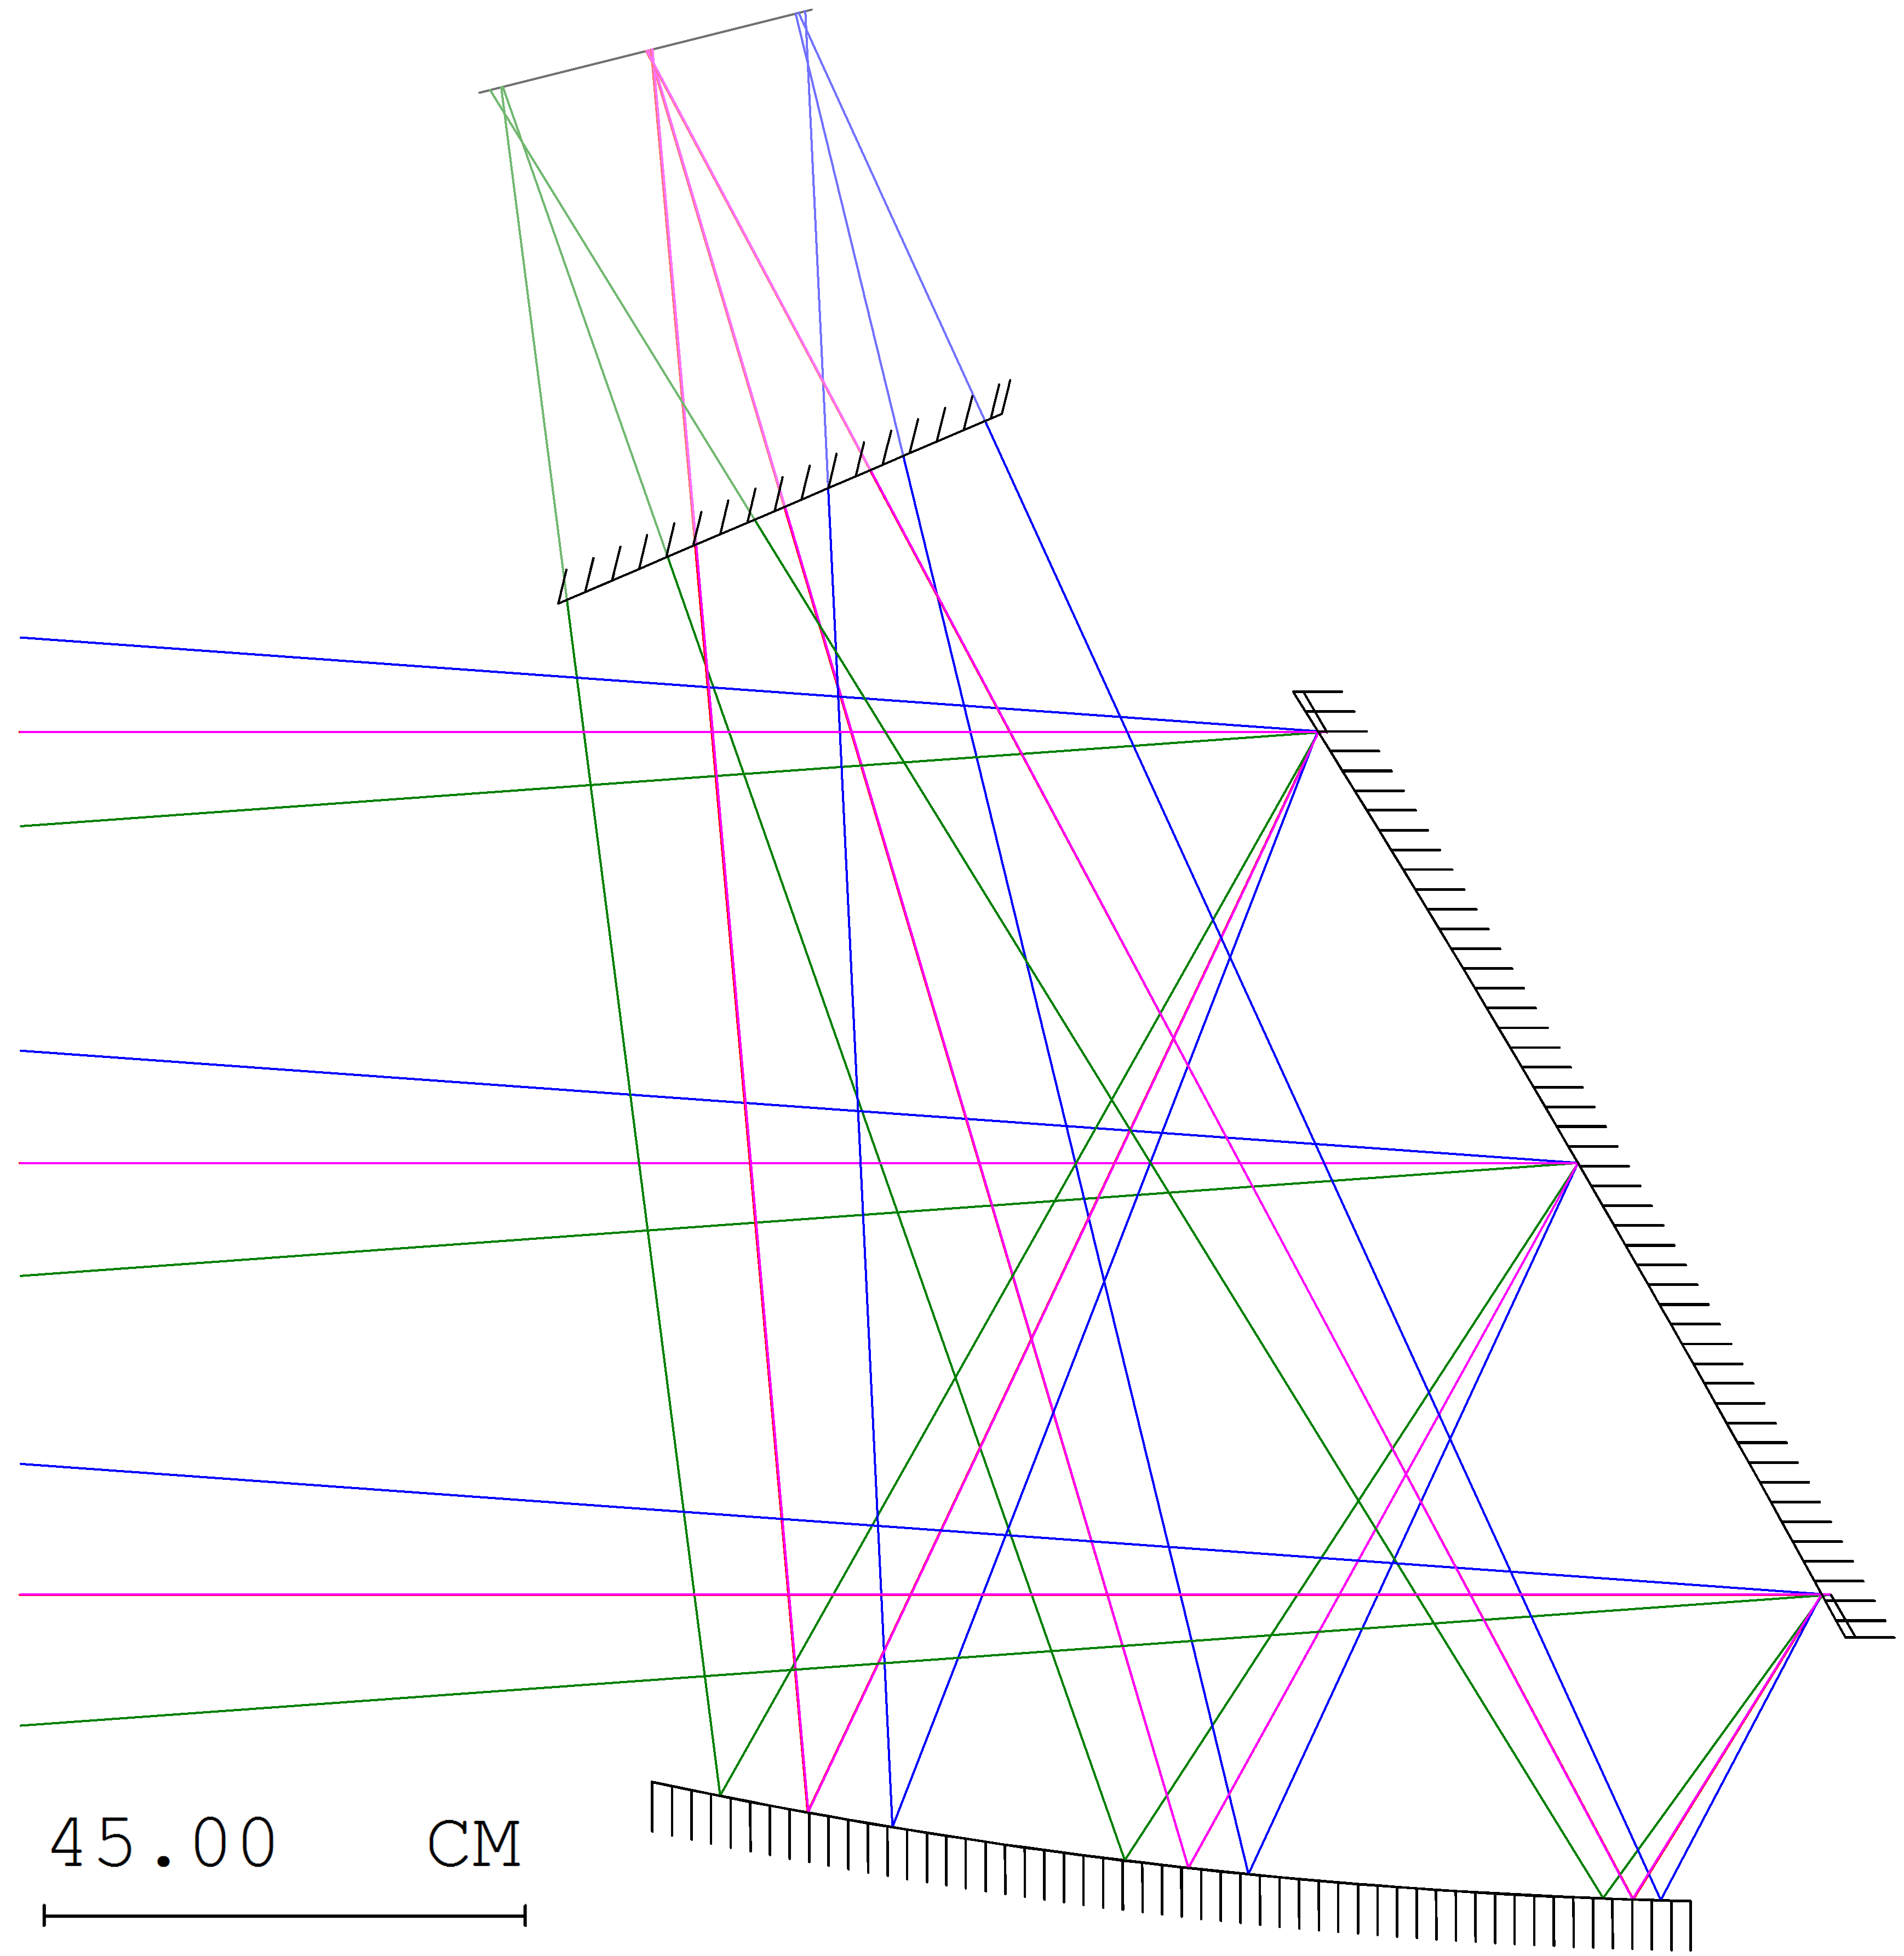
\includegraphics[width=0.3\textwidth]{xdragone_raytrace.png}\label{fig:dragone_ray}}
	\hfill
	\subfloat[CAD model of the Crossed Dragone system.  The view is looking down the boresight of the telescope. The 
	primary is blue, the secondary orange, and the tertiary is red.  The focal plane is green and baffles are grey.
	Below the telescope the white sunshields and the satellite service module are shown.]{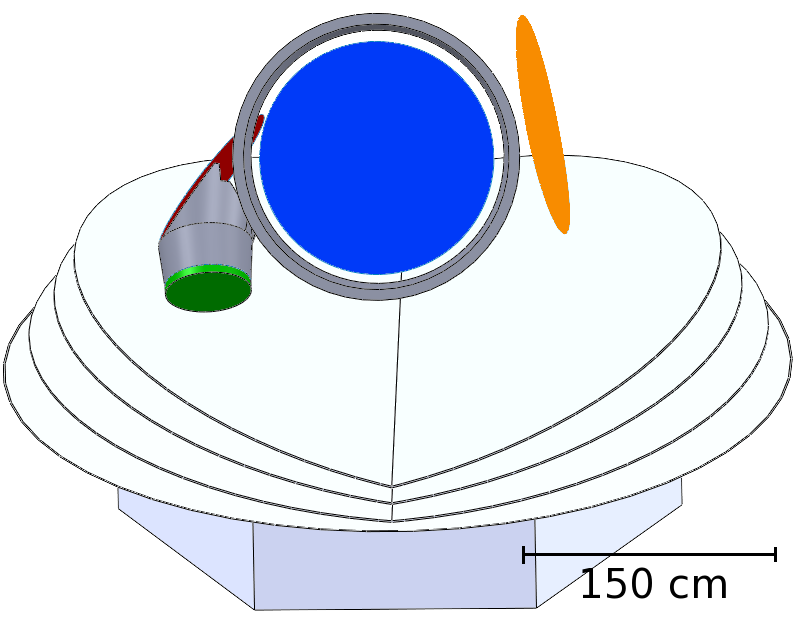
\includegraphics[width=0.3\textwidth]{full_xdragone.png}\label{fig:dragone_cad}}
	\caption{Ray trace and CAD models of the crossed-Dragone telescope proposed as the baseline for \coreplus. \comblue{I have left the drawings small, we could potentially squeeze in three side by side like in the last proposal to save space.}}
\end{figure}
%\begin{figure}[htbp] %  figure placement: here, top, bottom, or page
%	\includegraphics[width=12cm]{core_xdragone_strehl.png} 
%	\caption{Strehl$=0.8$ contours defining the diffraction limited field of view of \coreplus at 
%		160~GHz (yellow), 220~GHz (magenta), 340~GHz (cyan), 450~GHz (green), and 600~GHz (black). 
%		The usable field of view, limited by the ability to baffle the focal plane, is shown as a 
%		dashed blue circle.
%	}
%	\label{fig:strehl_xdragone}
%\end{figure}
This optical configuration is extremely promising for use with CMB instruments \comblue{Should we mention the likes of QUIET here?}, as it offers low sidelobe and spillover levels, excellent polarisation characteristics and naturally provides a wide diffraction limited field of view (DLFOV) and a flat, telecentric focal plane. The wide DLFOV means that a large focal plane can be realised (50~cm for this design), permitting the use of several thousand detectors which is critical in terms of realising the sensitivity requirements of the instrument for each observation band. For thermal, mass and cost reasons, such a high number of detectors renders the use of corrugated horns as the beam forming elements impractical. 
\begin{wraptable}{r}{10.5cm}
	\setlength{\belowcaptionskip}{-20pt}
	\begin{center}
		\begin{tabular}{@{\extracolsep{\fill}}c|c} 
			\toprule 
			\textbf{Parameter} & \textbf{Value } \\ \midrule
			\multicolumn{2}{c}{Crossed-Dragone (baseline for \coreplus ) } \\ \hline
			Primary mirror: projected diameter & 1.20 m \\
			Primary mirror: physical dimensions & 1.40 m $\times$ 1.30 m \\
			Secondary mirror dimensions & 1.40 m $\times$ 1.30 m \\
			Tertiary mirror dimensions & 0.80 m $\times$ 0.60 m \\
			Focal plane diameter & 0.50~m \\
			Telescope focal ratio (f\#)  & 2.54 \\ 
			%			Estimate of total mass & 53 kg \\  \hline
			Estimate of total mass & 90-100 kg \\  \hline
			\bottomrule
		\end{tabular}
		\caption{Parameters for the \coreplus\ telescope. The total mass is estimated by scaling from the 
			measured mass of the ALADIN telescope (a LIDAR mission for global measurement of vertical wind profiles), assuming an areal density of 28~kg/m\textsuperscript{3} for a primary mirror of diameter 1.5~m.}
		\label{tab:telparameters}
	\end{center}  
\end{wraptable}
The flat focal plane offered by this optical configuration, unlike the equivalent Gregorian design (used previously by missions such as \planck\ and \textit{WMAP} and considered at the ESA CDF study in 2016), allows the efficient tiling of the wafers necessary for planar antenna technology without the need to include a large tertiary lens in order to flatten the curved focal plane surface as in Gregorian designs, which would increase instrumental polarization and have implications for optical efficiency and absorption across the band. Such lenses are unavoidable in Gregorian designs if planar antennas are to be used, as the focal plane must be flattened to avoid the shadowing of neighbouring wafers. The naturally flat focal plane of the crossed-Dragone design was therefore a key factor in selecting it as the baseline option in place of an off-axis Gregorian. design\comblue{ESA wanted a Gregorian, based on the CDF. Their study treated the FPU as a blackbox and so they never considered this complication. Since that could be to the fore of their minds, is it okay to say this? Could we even put more emphasis on it?} The location of the focal plane, near the service module of the spacecraft, is also advantageous in terms of simplifying the electrical and cryogenic connections, minimizing the weight of the mechanical supports and reducing the moment of inertia of the satellite. The focal plane must be baffled in order to reject all stray light from the sky. Accounting for the proximity of the focal plane to the entrance aperture of the telescope, a possible baffling scheme is shown in figure \ref{fig:dragone_cad} which results in a focal plane of angular radius 4.6~deg in the azimuth direction and 4.8~deg in elevation. An additional benefit of this design is that the tertiary mirror could be easily replaced by a reflective active polarization modulator if one is deemed necessary.

Similar to \herschel\ and the \textit{ALADIN} instrument, the telescope mirrors are made from silicon carbide (SiC)\comblue{Does anything else need to be said about the mirrors? Perhaps it would be good to emphasise that this falls within the limits of what can be manufactured in one piece? I will also ask Jacques about what is being used as a basis for sensitivity calculations.}, with their shapes and offsets optimised to maximise the DLFOV across the \coreplus bandwidth, 60-600~GHz. Additionally, the telescope design is based on the Mizuguchi-Dragone condition which minimises cross-polarisation. The telescope optical train does not require lenses and so operates with nearly equal efficiency and negligible absorption over the entire frequency band. The contribution of the telescope to the instrumental polarization (the conversion of unpolarized light into polarized light by the instrument) at the edge of the focal plane where this effect will be the most pronounced, is of the order of -50~dB at 145~GHz \comblue{This figure relates purely to the impact of the three mirrors and does not include the mesh lenses/ antennas etc}. The polarization rotation (the amount by which the telescope rotates the orientation of the polarization) is also low and will be calibrated to the accuracy required prior to flight.

\comblue{We were going to prepare a few sentences on downscoping for inclusion in that section (3.8) but Jacques seems to have that covered, and the options don't really impact upon the telescope from the point of view of this section, other than one option being to use a 1~m mirror}
%A possible downscope option is to use a two mirror off-axis Gregorian design with a 1.2~m projected aperture. This was studied in detail and found to give rise to a focal plane which is approximately 4~deg in radius - %significantly smaller than that produced by the crossed-Dragone option. Additionally, the focal plane surface is naturally curved, and so if planar antenna technology is to be used then it is necessary to include an alumina %lens of diameter 44~cm which will have implications for instrumental polarization, optical efficiency and absorption across the band. The benefits of this optical configuration compared to the crossed-Dragone are a more %compact design with significantly smaller reflectors, and it is easier to baffle for stray light suppression. 

\end{document}